\chapter{Cars} \label{ch:cars}

Vehicles in \vvase{} are represented by .car files.  These files store all information that describes the vehicle itself, including suspension hardpoints, mass properties, etc.

When a new vehicle is created, defaults values for all properties are created such that the suspension takes a reasonable form.  This makes it easier to associate hardpoint names with the points shown on-screen.

When a car file is active, the \element{Main Display Area} contains a 3D rendering of the tires and suspension elements.  This rendering is described in \sref{sec:3dCarDisplay}.

Car files create several subsystems in the \element{Systems Tree}, with each subsystem having unique \element{Edit Panel} content.  These subsystems are described in \sref{sec:subsystems}.

\section{3D Car Display} \label{sec:3dCarDisplay}

The 3D vehicle rendering shows the locations of all of the suspension elements and tires in the specified kinematic state.  An example of the 3D rendering of a car is shown in \figref{fig:car}.  In the rendering, the green vectors represent roll centers and roll axes, and yellow vectors represent instant centers and instant axes.

\begin{figure}
  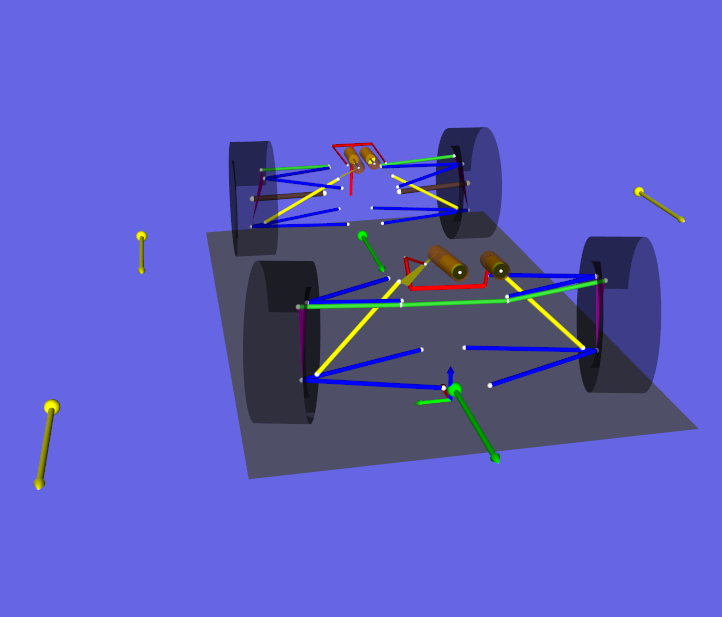
\includegraphics[width=\textwidth]{images/car}
  \caption{Example 3D car rendering for a kinematic state including roll and steer inputs} \label{fig:car}
  \centering
\end{figure}

It is possible to interact with the 3D display by clicking and dragging with the mouse to rotate, or using the mouse wheel to zoom.

By default, cars are rendered in perspective mode, but the \element{3D Toolbar} can be used to toggle between perspective and orthographic modes.  See \sref{ssec:3DToolbar} for more information.

The appearance of all of the suspension elements can be adjusted by clicking on the \element{Car} menu, and then selecting \button{Appearance Options}.  The color and size can be adjusted and the visibility of any object can be toggled on or off.  Resolution, which can also be adjusted, corresponds to the number of triangles used to approximate round objects during the rendering process.

When a hardpoint is selected in the \element{Edit Panel}, a ``helper orb'' is drawn, which highlights the selected point in the 3D display.  This can be helpful in understanding the naming of each hardpoint.

\section{Subsystems} \label{sec:subsystems}

Each car file includes several subsystems.  These subsystems can be accessed by expanding the active car in the Systems Tree.  The subsystems are described below.

\subsection{Aerodynamics} \label{ssec:aerodynamics}

This subsystem is currently unused.

\subsection{Brakes} \label{ssec:brakes}

The brakes subsystem includes three parameters that affect the calculated kinematic outputs.  These parameters are toggled to indicate whether or not the front and rear brakes are inboard or outboard, and the portion of the braking effort that can be expected to come from the front tires.  These parameters affect the calculation of the front anti-dive and rear anti-lift.

\subsection{Drivetrain} \label{ssec:drivetrain}

This subsystem is currently unused.

\subsection{Engine} \label{ssec:engine}

This subsystem is currently unused.

\subsection{Mass Properties} \label{ssec:massProperties}

There are several mass properties parameters associated with each car file.  For kinematics analysis, only the z-component of the center of gravity is currently used.  It affects only the calculation of the anti-dive and anti-lift values.

%For quasi-static analysis, all parameters except for the inertia tensor are used.

\subsection{Suspension} \label{ssec:suspension}

The suspension is the heart of the kinematics analysis.  This is where all of the suspension hardpoints are defined, as well as a number of other suspension geometry settings.  By default, the suspensions are assumed to be symmetric, but unchecking the corresponding option on the \element{Suspension} tab creates a separate additional tab for each corner instead of the \element{Front} and \element{Rear} tabs that exist by default.  Also on the \element{Suspension} tab are options for the type of anti-roll bar present at each end (if any) and whether or not \nth{3} springs are present at each end.  Depending on the selected anti-roll bar and \nth{3} spring options, a list of hardpoints may be displayed in the grid at the top of the panel.  These hardpoints can be edited by typing in new values in this grid.  Clicking on the hardpoint will highlight the corresponding point in the 3D display.

The additional tabs, whether there are two or four, are identical.  Each tab corresponds to a corner or a pair of corners at one end of the car and includes a list of hardpoints, spring/damper options and static toe and camber settings.  Just as with the \element{Suspension} tab, selecting a hardpoint in the list will highlight the corresponding hardpoint(s) in the 3D display.

By default, both ends of the car have pushrod suspensions.  By changing the \element{Attachment} to the \selection{Upper A-Arm} or a high location on the \selection{Upright} and modifying the bellcrank hardpoints, pullrods can also be modeled.  Outboard spring/damper units and rocker arms can be modeled by selecting the \selection{Outboard/Rocker} \element{Actuation Type}.

Static toe and camber settings affect only the calculated steer and camber values.

\subsection{Tires} \label{ssec:tires}

The diameter, width and stiffness of all four tires may be specified individually.  The width is for display purposes only.  The diameter affects the tire rendering as well as the kinematic calculations.  For the purposes of the kinematics analysis, the tires are assumed to be thin, rigid disks.  For all kinematic states the tires are assumed to rest on the ground.

For quasi-static analysis, the the tire stiffness parameters are used to compute tire deflections.  The rendering will still draw perfectly round tires, which will result in the tire being drawn slightly below the ground plane.
